%%%%%%%%%%%%%%%%%%%%%%%%%%%%%%%%%%%%%%%%%%%%%%%%%%%%%%%%%%%%%%%%%%
% The following comments were written in Portuguese, because this 
% template applies only for School of Technology at University 
% of Campinas, Brazil.
%
% Este é um modelo Latex para monografias de Trabalhos de Conclusão 
% de Curso (TCC) na graduação, monografias de Mestrado e Teses de 
% doutorado da Faculdade de Tecnologia (FT) da Universidade 
% Estadual de Campinas (UNICAMP).
%
% Esse modelo e seu respectivo arquivo de classe de documento 
% foram adaptados do modelo de teses e dissertações do 
% Instituto de Computação da UNICAMP e estão de acordo com a 
% Instrução Normativa CPG 002/2021.
%
% Autor: André Leon Sampaio Gradvohl, Dr.
% Email:     gradvohl@unicamp.br
% Lattes CV: http://lattes.cnpq.br/9343261628675642
% ORCID:     0000-0002-6520-9740
% 
% Última versão: 10/julho/2025.
%
% Adições/Alterações nesta última versão:
% - Ajustes na folha de aprovação.
%   - Simplificações na folha de aprovação por solicitação da Pró-reitoria de Pós-graduação
%%
%%%%%%%%%%%%%%%%%%%%%%%%%%%%%%%%%%%%%%%%%%%%%%%%%%%%%%%%%%%%%%%%%%
%
% Escolha: Portugues ou Ingles ou Espanhol.
% Para a versão final do texto, acrescente a palavra "Final".
\documentclass[Portugues,Final]{tese-FT}
%\documentclass[Ingles,Final]{tese-FT}
%\documentclass[Espanhol,Final]{tese-FT}
%
% Para uma compilação mais rápida, utilize a opção "Draft", em
% letras maiúsculas como a seguir. 
%\documentclass[Portugues,Draft]{tese-FT}
%
% Caso necessário, adicione também a opção "noFig". Essa opção 
% deixa de mostrar as figuras e, portanto, acelera mais ainda
% a compilação.
%\documentclass[Portugues,Draft,noFig]{tese-FT}
%
% Caso queira gerar uma versão para avaliação pelo Turnitin,
% (software utilizado pela Unicamp para emissão do relatório
% de originalidade), adicione a opção Turnitin conforme o 
% exemplo da linha a seguir:
%\documentclass[Portugues,Final,Turnitin]{tese-FT}

%Adicione seu arquivo com as referências bibliográficas
\addbibresource{bibliografia.bib}

%O pacote a seguir gera um "dummy text". Elimine a linha quando
% for editar seu texto.
\usepackage{lipsum}

\begin{document}

% Escolha entre autor ou autora:
\autor{Diego de Freitas Maia}
%\autora{Nome da Autora}

% Sempre deve haver um título em português:
\titulo{Análise de Desempenho em Processamento Hiperespectral para Sistemas Embarcados}

% Se a língua for o inglês ou o espanhol defina:
%\title{The Dissertation or Thesis Title in English or Spanish for FT}

% Escolha entre orientador ou orientadora e inclua os títulos:
\orientador{Prof.\ Dr.\ Leandro Ronchini Ximenes}
%\orientadora{Profa. Dra. Nome da Orientadora}

% Escolha entre coorientador ou coorientadora, se houver, 
% e inclua os títulos:
%\coorientador{Prof. Dr. Eng. Lic. Nome do Co-Orientador}
%\coorientadora{Prof. Dra. Eng. Lic. Nome da Co-Orientadora}

% Escolha entre uma das seis opções a seguir (comente as demais):
%\bsi         % para Trabalho de Conclusão de Curso em BSI
%\tads        % para Trabalho de Conclusão de Curso em TADS
%\qualificacaoMestrado  % Para textos de qualificação de mestrado.
%\qualificacaoDoutorado % Para textos de qualificação de doutorado.
\mestrado % para Dissertação de Mestrado em Tecnologia
%\doutorado  % para Tese de Doutorado em Tecnologia

%Defina a área de concentração. Se for TCC, deixe comentado.
\areaConcentracao{Sistemas de Informação e Comunicação}
%\areaConcentracao{Ambiente}
%\areaConcentracao{Ciência dos Materiais}

% Se houve cotutela, defina:
%\cotutela{Universidade Nova de Plutão}

% Defina a data da defesa no formato {Dia}{Mês}{Ano}
% Use apenas números! O template transformará em palavras,
% se necessário.
\datadadefesa{30}{12}{2025}

% Para a versão final defina:
% Repita o nome do Orientador(a) no primeiro avaliador
\avaliadorA{Prof.\ Dr.\ Leandro Ronchini Ximenes}{FT/UNICAMP}
\avaliadorB{Prof.ª Dr.ª Segunda Avaliadora}{Instituição da segunda avaliadora}
\avaliadorC{Dr. Terceiro Avaliador}{Instituição do terceiro avaliador}
% \avaliadorD{Prof. Dr. Quarto Avaliador}{Instituição do quarto avaliador}
% \avaliadorE{Prof. Dr. Quinto Avaliador}{Instituição do quinto avaliador}
% \avaliadorF{Prof. Dr. Sexto Avaliador}{Instituição do sexto avaliador}
% \avaliadorG{Prof. Dr. Sétimo Avaliador}{Instituição do sétimo avaliador}
% \avaliadorH{Prof. Dr. Oitavo Avaliador}{Instituição do oitavo avaliador}

% Para incluir a ficha catalográfica em PDF na versão final, 
% copie o arquivo PDF para o projeto no Overleaf, descomente 
% e informe o nome do arquivo no comando a seguir.
%\fichacatalografica{SeuArquivo.pdf}
% OBSERVAÇÂO: O comando para a ficha catalográfica só é válido 
% versoes finais de TCC, teses e dissertações (não é válido para qualificação 
% ou TCCs que não serão disponibilizados na biblioteca).
%
% Para deixar uma página em branco no lugar da ficha 
% catalográfica, descomente uma das três linhas a seguir:
%\fichacatalografica{branco.pdf} % Português
%\fichacatalografica{white.pdf}  % Inglês
%\fichacatalografica{blanco.pdf} % Espanhol

% Este comando deve ficar aqui:
\paginasiniciais

% Se houver uma dedicatória, informe no comando a seguir. 
% A dedicatória deve ter poucas linhas.
 %\dedicatoria{A dedicatória deve ocupar poucas linhas.}
 
% Se houver epígrafe, use o comando \epigrafe a seguir
%   - O primeiro parâmetro é o autor dos dizeres.
%   - O segundo parâmetro são os dizeres.
% \epigrafe{Hippocrates}{
% {\it
% Vita brevis,\\
% ars longa,\\
% occasio praeceps,\\
% experimentum periculosum,\\
% iudicium difficile.}
% }

% O comando condicional \ifturnitin a seguir é importante para 
% preparar o texto para encaminhamento ao Turnitin. 
% NÃO REMOVA!!
% O \fi correspondente está após o comando \tableofcontents
\ifturnitin
   \relax 
\else
% Adicione no arquivo "agradecimentos.tex" os seus agradecimentos
% Caso prefira omitir os agradecimentos, comente a linha a seguir.
% \prefacesection{Agradecimentos}
Coloque nesse arquivo os agradecimentos àqueles que o ajudaram no seu trabalho. Os agradecimentos devem ocupar uma única página. Não esqueça de adicionar a frase a seguir.

O presente trabalho foi realizado com apoio da Coordenação de Aperfeiçoamento de Pessoal de Nível Superior -- Brasil (CAPES) -- Código de Financiamento 001.

% Sempre deve haver um resumo em português:
\begin{resumo}
O resumo deve ter no máximo 500 palavras e deve ocupar uma única página.
\end{resumo}

% Sempre deve haver um abstract:
\begin{abstract}
The abstract must have at most 500 words and must fit in a single page.
\end{abstract}

% Se houver um resumo em espanhol, descomente as linhas a seguir:
%\begin{resumen}
% A mesma regra aplica-se.
%\end{resumen}

% A lista de figuras:
\listoffigures

% A lista de tabelas:
\listoftables

% A lista de símbolos é opcional. Não confunda a lista de símbolos 
% matemáticos com a lista de abreviaturas (que vem depois).
\prefacesection{Lista de Símbolos}

% Coloque o símbolo na primeira coluna e a 
% descrição na segunda coluna. Use descrições
% rápidas.

\begin{table}[!ht]
  \begin{tabular}{p{1cm}p{14cm}}
	$\alpha$  & Descrição do símbolo $\alpha$. utilize uma descrição curta. De preferência, que ocupe no máximo uma linha.\\
	$\beta$   & Descrição do símbolo $\beta$. \\
	$\gamma$  & Descrição do símbolo $\gamma$. 
  \end{tabular}
\end{table}

% A lista de abreviações e siglas vem a seguir.
% Dê uma olhada no pacote nomencl para ver os comandos para 
% adicionar abreviações e siglas no texto.
% Foram adicionados os comandos \Sigla{Sigla por extenso}{abrev} e 
% \SiglaHifen{Sigla por extenso}{abrev} para adicionar as siglas 
% diretamente no texto e criar a lisa de abreviaturas 
% automaticamente
\printnomenclature[3cm]

% O sumário vem aqui:
\tableofcontents

%% O comando \fi a seguir é obrigatório para o controle 
%% da opção "turnitin". Não o remova!!
\fi

% E a linha a seguir deve ficar bem aqui. Não mude.
\fimdaspaginasiniciais

% O corpo da dissertação ou tese começa aqui:
%
% O comando a seguir inclui o arquivo introducao.tex
% que contém o capítulo de Introdução. 
% Detalhe: não precisa incluir a extensão .tex
% Aqui começa o capítulo de Introdução.
% Use o comando \label para definir um rótulo, 
% caso seja necessário referenciar esse capítulo
% posteriormente.
\chapter{Introdução}\label{chp:Introducao}

% Contextualização do problema baseada na nova proposta
O processamento de dados hiperespectrais representa um desafio computacional significativo, especialmente em aplicações de tempo real que demandam alta precisão e eficiência energética. Com o crescimento exponencial da utilização de sensores hiperespectrais em aplicações agrícolas e ambientais, a necessidade por arquiteturas computacionais otimizadas que possam processar grandes volumes de dados espectrais em tempo real tornou-se crítica para viabilizar aplicações práticas efetivas.

O processamento hiperespectral pode ser realizado em diferentes arquiteturas computacionais, cada uma com suas características e trade-offs específicos. Processadores de propósito geral (CPUs) oferecem flexibilidade e facilidade de programação, unidades de processamento gráfico (GPUs) proporcionam paralelismo massivo, e FPGAs (Field-Programmable Gate Arrays) permitem customização de hardware com alta eficiência energética. A escolha da arquitetura mais adequada para uma aplicação específica requer uma análise aprofundada das características e requisitos do processamento hiperespectral em tempo real.

Adicionalmente, a possibilidade de combinar diferentes tecnologias em arquiteturas híbridas emerge como uma alternativa para potencialmente superar limitações individuais de cada processador. A integração estratégica de diferentes arquiteturas pode oferecer oportunidades para otimização de desempenho em cenários específicos, embora também introduza desafios adicionais de complexidade e gerenciamento de recursos.

\section{Motivação}\label{sec:motivacao}

A motivação para esta pesquisa deriva de múltiplos fatores convergentes que destacam a importância de uma análise sistemática e comparativa das diferentes arquiteturas de processamento para aplicações hiperespectrais em tempo real:

\subsection{Desafios Computacionais do Processamento Hiperespectral}
O processamento de dados hiperespectrais apresenta características únicas que demandam soluções computacionais especializadas. Cada pixel hiperespectral contém informações de centenas de bandas espectrais, resultando em volumes de dados que podem exceder terabytes em aplicações típicas. O processamento dessas informações envolve operações computacionalmente intensivas, incluindo correções atmosféricas, redução de dimensionalidade, classificação e análise de padrões espectrais.

Os algoritmos de processamento hiperespectral apresentam diferentes características computacionais que podem se beneficiar de diferentes arquiteturas de processamento. A natureza das operações varia desde cálculos simples e altamente paralelizáveis até algoritmos complexos com dependências de dados significativas, criando um cenário desafiador para a seleção da arquitetura mais apropriada.

\subsection{Características das Arquiteturas de Processamento}
Cada arquitetura de processamento apresenta características distintas que podem ser mais ou menos adequadas para diferentes aspectos do processamento hiperespectral:

\begin{itemize}
    \item \textbf{CPU (Processadores de Propósito Geral)}:
    \begin{itemize}
        \item Flexibilidade e facilidade de programação
        \item Bom desempenho em operações sequenciais
        \item Suporte a instruções vetoriais avançadas
        \item Limitações em paralelismo massivo
    \end{itemize}
    
    \item \textbf{GPU (Unidades de Processamento Gráfico)}:
    \begin{itemize}
        \item Excelente para paralelismo massivo
        \item Alto throughput em operações de ponto flutuante
        \item Otimizado para processamento de dados regulares
        \item Consumo energético significativo
    \end{itemize}
    
    \item \textbf{FPGA (Field-Programmable Gate Arrays)}:
    \begin{itemize}
        \item Alta eficiência energética
        \item Customização de hardware para operações específicas
        \item Excelente para operações de baixa latência
        \item Complexidade de desenvolvimento maior
    \end{itemize}
\end{itemize}

\subsection{Necessidade de Análise Comparativa}
A diversidade de arquiteturas disponíveis e a complexidade das aplicações hiperespectrais criam uma necessidade crítica por:

\begin{itemize}
    \item Avaliação sistemática de desempenho em diferentes cenários
    \item Análise objetiva de trade-offs entre arquiteturas
    \item Compreensão dos impactos em eficiência energética
    \item Identificação de casos de uso ideais para cada arquitetura
\end{itemize}

\section{Objetivos}\label{sec:objetivos}

\subsection{Objetivo Geral}
Realizar uma análise comparativa abrangente de diferentes arquiteturas computacionais (CPU, GPU e FPGA) para processamento de imagens hiperespectrais em tempo real, com foco em aplicações agrícolas e monitoramento ambiental, estabelecendo métricas objetivas de desempenho, eficiência energética e precisão para cada arquitetura em diferentes cenários de aplicação, incluindo uma investigação adicional sobre o potencial de arquiteturas híbridas.

\subsection{Objetivos Específicos}
\begin{enumerate}
    \item \textbf{Caracterizar operações}: Analisar e classificar operações de processamento hiperespectral:
    \begin{itemize}
        \item Complexidade computacional
        \item Requisitos de paralelismo
        \item Padrões de acesso à memória
        \item Dependências de dados
    \end{itemize}
    
    \item \textbf{Implementar algoritmos otimizados}: Desenvolver implementações específicas para cada arquitetura:
    \begin{itemize}
        \item CPU: Otimizações vetoriais e multi-thread
        \item GPU: Implementações CUDA otimizadas
        \item FPGA: Designs VHDL customizados
    \end{itemize}
    
    \item \textbf{Desenvolver framework de simulação}: Criar ambiente controlado para:
    \begin{itemize}
        \item Geração de dados de teste
        \item Medição de métricas
        \item Validação de resultados
        \item Análise comparativa
    \end{itemize}
    
    \item \textbf{Realizar análise comparativa}: Avaliar cada arquitetura em termos de:
    \begin{itemize}
        \item Desempenho computacional
        \item Eficiência energética
        \item Precisão dos resultados
        \item Complexidade de implementação
    \end{itemize}
    
    \item \textbf{Investigar arquiteturas híbridas}: Analisar potenciais benefícios de:
    \begin{itemize}
        \item Combinações de processadores
        \item Estratégias de particionamento
        \item Trade-offs de integração
        \item Cenários de aplicação específicos
    \end{itemize}
    
    \item \textbf{Validar em aplicações reais}: Testar em cenários práticos:
    \begin{itemize}
        \item Datasets hiperespectrais padrão
        \item Aplicações agrícolas específicas
        \item Monitoramento ambiental em tempo real
    \end{itemize}
    
    \item \textbf{Desenvolver diretrizes de seleção}: Estabelecer critérios para:
    \begin{itemize}
        \item Escolha de arquitetura apropriada
        \item Otimizações específicas por cenário
        \item Considerações de implementação
        \item Análise de custo-benefício
    \end{itemize}
\end{enumerate}

\section{Contribuições Esperadas}\label{sec:contribuicoes}

Esta pesquisa visa contribuir para o avanço do estado da arte em processamento hiperespectral através de:

\subsection{Contribuições Metodológicas}
\begin{enumerate}
    \item \textbf{Framework de avaliação}: Metodologia sistemática para:
    \begin{itemize}
        \item Caracterização de operações
        \item Análise de arquiteturas
        \item Medição de desempenho
        \item Comparação objetiva
    \end{itemize}
    
    \item \textbf{Métricas de comparação}: Definição de indicadores para:
    \begin{itemize}
        \item Desempenho computacional
        \item Eficiência energética
        \item Qualidade de resultados
        \item Complexidade de implementação
    \end{itemize}
\end{enumerate}

\subsection{Contribuições Técnicas}
\begin{enumerate}
    \item \textbf{Implementações otimizadas}: Desenvolvimento de:
    \begin{itemize}
        \item Algoritmos CPU vetorizados
        \item Kernels GPU eficientes
        \item Designs FPGA customizados
        \item Integrações híbridas
    \end{itemize}
    
    \item \textbf{Framework de simulação}: Ferramentas para:
    \begin{itemize}
        \item Geração de dados
        \item Medição de métricas
        \item Validação de resultados
        \item Análise comparativa
    \end{itemize}
\end{enumerate}

\subsection{Contribuições Práticas}
\begin{enumerate}
    \item \textbf{Guia de seleção}: Diretrizes para escolha de:
    \begin{itemize}
        \item Arquitetura apropriada
        \item Otimizações específicas
        \item Estratégias de implementação
        \item Considerações de custo
    \end{itemize}
    
    \item \textbf{Análise de viabilidade}: Avaliação de:
    \begin{itemize}
        \item Custo-benefício
        \item Complexidade de desenvolvimento
        \item Requisitos de recursos
        \item Potencial de escalabilidade
    \end{itemize}
\end{enumerate}

\section{Organização do Texto}\label{sec:organizacao}

Esta dissertação está estruturada em sete capítulos:

\begin{itemize}
    \item \textbf{Capítulo 2 - Levantamento Bibliográfico}: Apresenta revisão da literatura sobre processamento hiperespectral, arquiteturas de processamento, técnicas de otimização e aplicações em tempo real.
    
    \item \textbf{Capítulo 3 - Metodologia}: Detalha a metodologia de avaliação, incluindo caracterização de operações, framework de simulação, métricas de avaliação e protocolos experimentais.
    
    \item \textbf{Capítulo 4 - Implementações}: Descreve as implementações otimizadas para cada arquitetura (CPU, GPU, FPGA) e considerações sobre integrações híbridas.
    
    \item \textbf{Capítulo 5 - Resultados}: Apresenta resultados experimentais comparativos, incluindo análises de desempenho, eficiência energética e qualidade.
    
    \item \textbf{Capítulo 6 - Discussão}: Analisa os resultados obtidos, discute trade-offs identificados e propõe diretrizes de seleção de arquitetura.
    
    \item \textbf{Capítulo 7 - Conclusões}: Sumariza as contribuições, limitações e recomendações para trabalhos futuros.
\end{itemize}

\section{Infraestrutura Experimental}\label{sec:infraestrutura}

A validação experimental será realizada utilizando:

\subsection{Plataformas de Desenvolvimento}
\begin{itemize}
    \item \textbf{CPU}: Processador multi-core com suporte AVX-512
    \item \textbf{GPU}: NVIDIA GPU com suporte CUDA
    \item \textbf{FPGA}: Simulação via GHDL e síntese em hardware quando disponível
    \item \textbf{Ambiente}: Linux com ferramentas de desenvolvimento e análise
\end{itemize}

\subsection{Datasets de Validação}
\begin{itemize}
    \item \textbf{Sintéticos}: Datasets gerados para testes controlados
    \item \textbf{Benchmark}: Indian Pines, Pavia University
    \item \textbf{Reais}: Datasets agrícolas e ambientais específicos
\end{itemize}

\subsection{Métricas de Avaliação}
\begin{itemize}
    \item \textbf{Desempenho}: Throughput, latência, utilização de recursos
    \item \textbf{Energia}: Consumo, eficiência, perfil térmico
    \item \textbf{Qualidade}: Precisão, SNR, estabilidade
    \item \textbf{Desenvolvimento}: Complexidade, tempo, manutenibilidade
\end{itemize}

A próxima seção estabelece a fundamentação teórica necessária para compreensão das tecnologias envolvidas e do estado da arte em processamento hiperespectral em tempo real.

% O comando a seguir inclui o arquivo levantamento.tex
% que contém o capítulo de levantamento bibliográfico. 
% Detalhe: não precisa incluir a extensão .tex
\chapter{Levantamento bibliográfico}\label{chp:levantamento}
% O comando a seguir gera um "dummy text". 
% Elimine-o quando escrever sua dissertação.
\lipsum[6]


% O comando a seguir inclui o arquivo desenvolvimento.tex
% que contém o capítulo de desenvolvimento. 
% Detalhe: não precisa incluir a extensão .tex
%% Capítulo 3: Metodologia de Validação
%% Focado na Validação Conceitual e Metodológica da Etapa 1

\section{Visão Geral da Metodologia de Validação}

Esta pesquisa adota uma metodologia de \textbf{validação conceitual} estruturada em quatro fases para avaliar o potencial de integração de técnicas comprovadas em sistemas heterogêneos para processamento hiperespectral embarcado. O objetivo é estabelecer bases metodológicas sólidas através de análise sistemática, modelagem teórica e protótipos de prova de conceito.

A metodologia de validação baseia-se em três pilares fundamentais: \textbf{(1)} análise sistemática da literatura para catalogação de técnicas comprovadas, \textbf{(2)} modelagem e simulação para quantificação de trade-offs, e \textbf{(3)} protótipos conceituais para validação experimental dos conceitos mais promissores.

\section{Framework Arquitetural Conceitual}

\subsection{Modelo de Sistema Heterogêneo}

Para fins de validação conceitual, define-se um modelo de sistema heterogêneo com pipeline de três estágios especializados que servirá como base para simulações e análises:

\begin{enumerate}
\item \textbf{Estágio de Pré-processamento (FPGA)}: Correção radiométrica, seleção de bandas e compressive sensing
\item \textbf{Estágio de Processamento (GPU)}: Reconstrução de dados e extração de características
\item \textbf{Estágio de Classificação (CPU)}: Algoritmos de classificação e controle do sistema
\end{enumerate}

\subsection{Plataforma de Referência para Modelagem}

A modelagem teórica baseia-se em uma plataforma de referência representativa do estado da arte em sistemas embarcados:
\begin{itemize}
\item \textbf{Processamento}: ARM Cortex-A78 + NVIDIA Jetson Orin + Xilinx Zynq UltraScale+
\item \textbf{Memória}: 16GB LPDDR5 compartilhada
\item \textbf{Orçamento Energético}: 15W TDP total
\item \textbf{Throughput Alvo}: >25 fps para imagens 614×512×224 bandas
\end{itemize}

Esta configuração baseia-se em validações experimentais da literatura \cite{diaz2019, hwang2011} e representa o estado da arte atual em plataformas heterogêneas embarcadas.

\subsection{Estudo de Caso Industrial: SightLine Applications}

Para contextualizar a aplicação prática dos conceitos de computação heterogênea, analisa-se o caso da \textbf{SightLine Applications}, uma empresa líder no fornecimento de soluções de processamento de vídeo embarcado para aplicações de Inteligência, Vigilância e Reconhecimento (ISR), especialmente em Veículos Aéreos Não Tripulados (VANTs). As soluções da empresa precisam operar com restrições severas de Tamanho, Peso e Potência (SWaP), tornando a eficiência energética um requisito fundamental.

O produto de destaque da empresa, o processador de vídeo \textbf{4100-OEM}, é um exemplo claro de um sistema heterogêneo. Ele é baseado no System-on-Module (SOM) \textbf{Open-Q 8250CS} da Lantronix, que utiliza o SoC \textbf{Qualcomm QCS8250} \cite{lantronix2023openq}. A arquitetura deste SoC é intrinsecamente heterogênea, distribuindo as cargas de trabalho entre múltiplos núcleos de processamento especializados:

\begin{itemize}
    \item \textbf{CPU Octa-core Kryo™ 585}: Unidade baseada em ARM Cortex, responsável pelo sistema operacional, controle de fluxo, e tarefas de gerenciamento geral.
    \item \textbf{GPU Adreno™ 650}: Acelerador gráfico para processamento massivamente paralelo, ideal para tarefas como renderização, filtragem de imagem e transformações geométricas.
    \item \textbf{DSP Hexagon™}: Processador de Sinal Digital com extensões vetoriais, otimizado para algoritmos matemáticos de baixa latência, como estabilização de imagem e processamento de sinais de sensores.
    \item \textbf{NPU (Neural Processing Unit)}: Um motor de IA dedicado, capaz de executar até 15 trilhões de operações por segundo (TOPS), acelerando cargas de trabalho de \textit{deep learning} para detecção e classificação de objetos em tempo real.
    \item \textbf{ISP (Image Signal Processor) Spectra™ 480}: Unidade dedicada ao pipeline de processamento de imagem, lidando com tarefas como demosaicing, balanço de branco e redução de ruído diretamente do sensor.
\end{itemize}

A abordagem da SightLine, ao adotar um SoC heterogêneo como o QCS8250, permite que cada componente do pipeline de processamento de vídeo seja executado no núcleo mais eficiente para aquela tarefa específica. Isso resulta em um sistema de alta performance, capaz de processar múltiplos streams de vídeo em alta resolução com baixa latência e, crucialmente, dentro de um envelope de consumo energético extremamente restrito (tipicamente entre 5W e 15W). Este estudo de caso valida a premissa de que a computação heterogênea não é apenas uma construção teórica, but uma necessidade prática para a próxima geração de sistemas embarcados inteligentes.


\section{Fase 1: Análise Sistemática do Estado da Arte (2 meses)}

\subsection{Catalogação de Técnicas Comprovadas}

Esta fase concentra-se na análise sistemática da literatura para catalogar e caracterizar técnicas comprovadas de otimização para processamento hiperespectral embarcado:

\textbf{Objetivos Específicos}:
\begin{itemize}
\item Catalogação sistemática de técnicas de redução de dados (compressive sensing, seleção de bandas)
\item Análise de algoritmos de otimização energética e codesign HW/SW
\item Caracterização de implementações heterogêneas (CPU/GPU/FPGA) da literatura
\item Identificação de lacunas e oportunidades de integração
\end{itemize}

\textbf{Metodologia de Análise}:
\begin{itemize}
\item \textbf{Revisão Sistemática}: Análise de 20+ artigos científicos com critérios de seleção definidos
\item \textbf{Matriz de Caracterização}: Organização das técnicas por categoria (redução de dados, otimização energética, codesign)
\item \textbf{Análise Quantitativa}: Extração de métricas de performance, consumo e precisão da literatura
\item \textbf{Identificação de Lacunas}: Mapeamento de oportunidades para integração sistemática
\end{itemize}

\subsection{Estabelecimento de Baselines}

\textbf{Datasets de Validação}:
Baseados nas referências da literatura \cite{lou2024, ullah2020}:
\begin{itemize}
\item \textbf{AVIRIS Indian Pines}: Dataset padrão (145×145×220) para agricultura
\item \textbf{Pavia University}: Ambiente urbano (610×340×103) para robustez
\item \textbf{Salinas Valley}: Agricultura diversificada (512×217×224)
\end{itemize}

\textbf{Métricas de Avaliação}:
\begin{itemize}
\item \textbf{Performance}: Throughput (fps), latência (ms/pixel), utilização recursos (%)
\item \textbf{Energética}: Consumo total (W), eficiência energética (fps/W)
\item \textbf{Qualidade}: Precisão (%), recall (%), F1-score, kappa coefficient
\end{itemize}

\section{Fase 2: Modelagem e Simulação Conceitual (3 meses)}

\subsection{Modelagem Teórica das Técnicas}

Esta fase desenvolve modelos matemáticos e simulações para validar o potencial das técnicas identificadas na Fase 1:

\subsubsection{Modelagem de Técnicas de Redução de Dados}

\begin{itemize}
\item \textbf{Compressive Sensing}: Modelagem da redução de 50-70\% dos dados (Lim et al.) com análise de trade-offs precisão vs compressão
\item \textbf{Seleção EMCR}: Simulação da redução de 80\% das bandas mantendo 99.7\% de precisão (Martins et al.)
\item \textbf{Codesign HW/SW}: Modelagem do potencial de melhoria energética de 43.5x (Hwang et al.)
\end{itemize}

\textbf{Objetivo}: Quantificar através de simulações o potencial teórico de cada técnica e suas combinações.

\subsubsection{Simulação de Trade-offs}

Desenvolvimento de simuladores para análise quantitativa dos trade-offs:

\begin{itemize}
\item \textbf{Simulador de Consumo Energético}: Modelo baseado em medições da literatura para estimar consumo por módulo
\item \textbf{Simulador de Latência}: Análise de pipeline com diferentes configurações de paralelização
\item \textbf{Simulador de Precisão}: Avaliação do impacto das reduções de dados na qualidade final
\end{itemize}

\subsection{Análise de Sensibilidade}

\textbf{Parâmetros de Análise}:
\begin{itemize}
\item Taxa de compressão do compressive sensing (10-70\%)
\item Número de bandas selecionadas EMCR (20-100 bandas)
\item Particionamento de carga entre módulos (0-100\% por módulo)
\item Precisão de ponto flutuante (FP16, FP32, INT8)
\end{itemize}

\textbf{Métricas de Saída}:
\begin{itemize}
\item Consumo energético estimado por configuração
\item Latência teórica end-to-end
\item Precisão de classificação esperada
\item Throughput máximo alcançável
\end{itemize}

\section{Fase 3: Protótipos de Prova de Conceito (3 meses)}

\subsection{Implementação de Protótipos Simplificados}

Esta fase implementa protótipos simplificados das técnicas mais promissoras para validação experimental dos conceitos:

\subsubsection{Protótipo de Compressive Sensing}

\begin{itemize}
\item \textbf{Plataforma}: MATLAB/Python com bibliotecas otimizadas
\item \textbf{Objetivo}: Validar experimentalmente as reduções teóricas de dados
\item \textbf{Métricas}: Taxa de compressão vs precisão de reconstrução
\end{itemize}

\subsubsection{Protótipo de Seleção EMCR}

\begin{itemize}
\item \textbf{Plataforma}: Python com scikit-learn otimizado
\item \textbf{Objetivo}: Confirmar redução de processamento mantendo precisão
\item \textbf{Métricas}: Número de bandas vs precisão de classificação
\end{itemize}

\subsubsection{Protótipo de Pipeline Heterogêneo}

\begin{itemize}
\item \textbf{Plataforma}: Simulação em MATLAB Simulink
\item \textbf{Objetivo}: Avaliar coordenação entre módulos e balanceamento de carga
\item \textbf{Métricas}: Utilização de recursos vs throughput total
\end{itemize}

\subsection{Validação Experimental}

\textbf{Protocolo de Teste}:
\begin{enumerate}
\item Execução de cada protótipo nos datasets de referência
\item Medição das métricas de performance, consumo e qualidade
\item Comparação com baselines da literatura
\item Análise de variabilidade e robustez dos resultados
\end{enumerate}

\textbf{Critérios de Validação}:
\begin{itemize}
\item Confirmação das métricas reportadas na literatura
\item Identificação de fatores limitantes não reportados
\item Quantificação da variabilidade entre diferentes datasets
\end{itemize}

\section{Fase 4: Framework Arquitetural e Diretrizes (2 meses)}

\subsection{Consolidação dos Resultados}

Esta fase consolida os resultados das fases anteriores em um framework arquitetural conceitual para orientar a implementação futura:

\subsubsection{Framework de Decisão}

Desenvolvimento de um framework para seleção de técnicas baseado em:
\begin{itemize}
\item \textbf{Características da Aplicação}: Requisitos de latência, precisão e consumo
\item \textbf{Restrições da Plataforma}: Recursos disponíveis e orçamento energético
\item \textbf{Características dos Dados}: Resolução espacial/espectral e complexidade da cena
\end{itemize}

\subsubsection{Especificações Técnicas}

Definição de especificações técnicas para a implementação na Etapa 2:
\begin{itemize}
\item \textbf{Arquitetura do Sistema}: Configuração otimizada dos módulos heterogêneos
\item \textbf{Protocolos de Comunicação}: Interfaces entre módulos FPGA/GPU/CPU
\item \textbf{Algoritmos Adaptativos}: Estratégias de ajuste dinâmico de qualidade vs recursos
\item \textbf{Métricas de Monitoramento}: Indicadores para controle em tempo real
\end{itemize}

\subsection{Diretrizes para a Etapa 2}

\textbf{Recomendações Arquiteturais}:
\begin{itemize}
\item Configuração ótima de módulos baseada na análise de trade-offs
\item Estratégias de implementação prioritárias
\item Riscos identificados e estratégias de mitigação
\end{itemize}

\textbf{Plano de Implementação}:
\begin{itemize}
\item Sequência de desenvolvimento dos módulos
\item Milestones de validação intermediária
\item Critérios de sucesso quantitativos
\end{itemize}

\section{Cronograma de Execução}

\subsection{Visão Geral do Cronograma}

O desenvolvimento desta pesquisa está estruturado em um cronograma detalhado de 14 meses, iniciando em agosto de 2025 e culminando com a defesa em setembro de 2026. O cronograma foi organizado em quatro etapas principais, cada uma com objetivos específicos e entregáveis bem definidos.

A Figura \ref{fig:cronograma} apresenta uma visualização detalhada do cronograma de execução, incluindo as dependências entre tarefas, milestones críticos e o progresso atual do projeto. Esta visualização também está disponível no arquivo \texttt{cronograma\_mestrado\_gantt.html} e permite acompanhar o progresso em tempo real através de uma interface interativa desenvolvida com D3.js.

\begin{figure}[htbp]
\centering
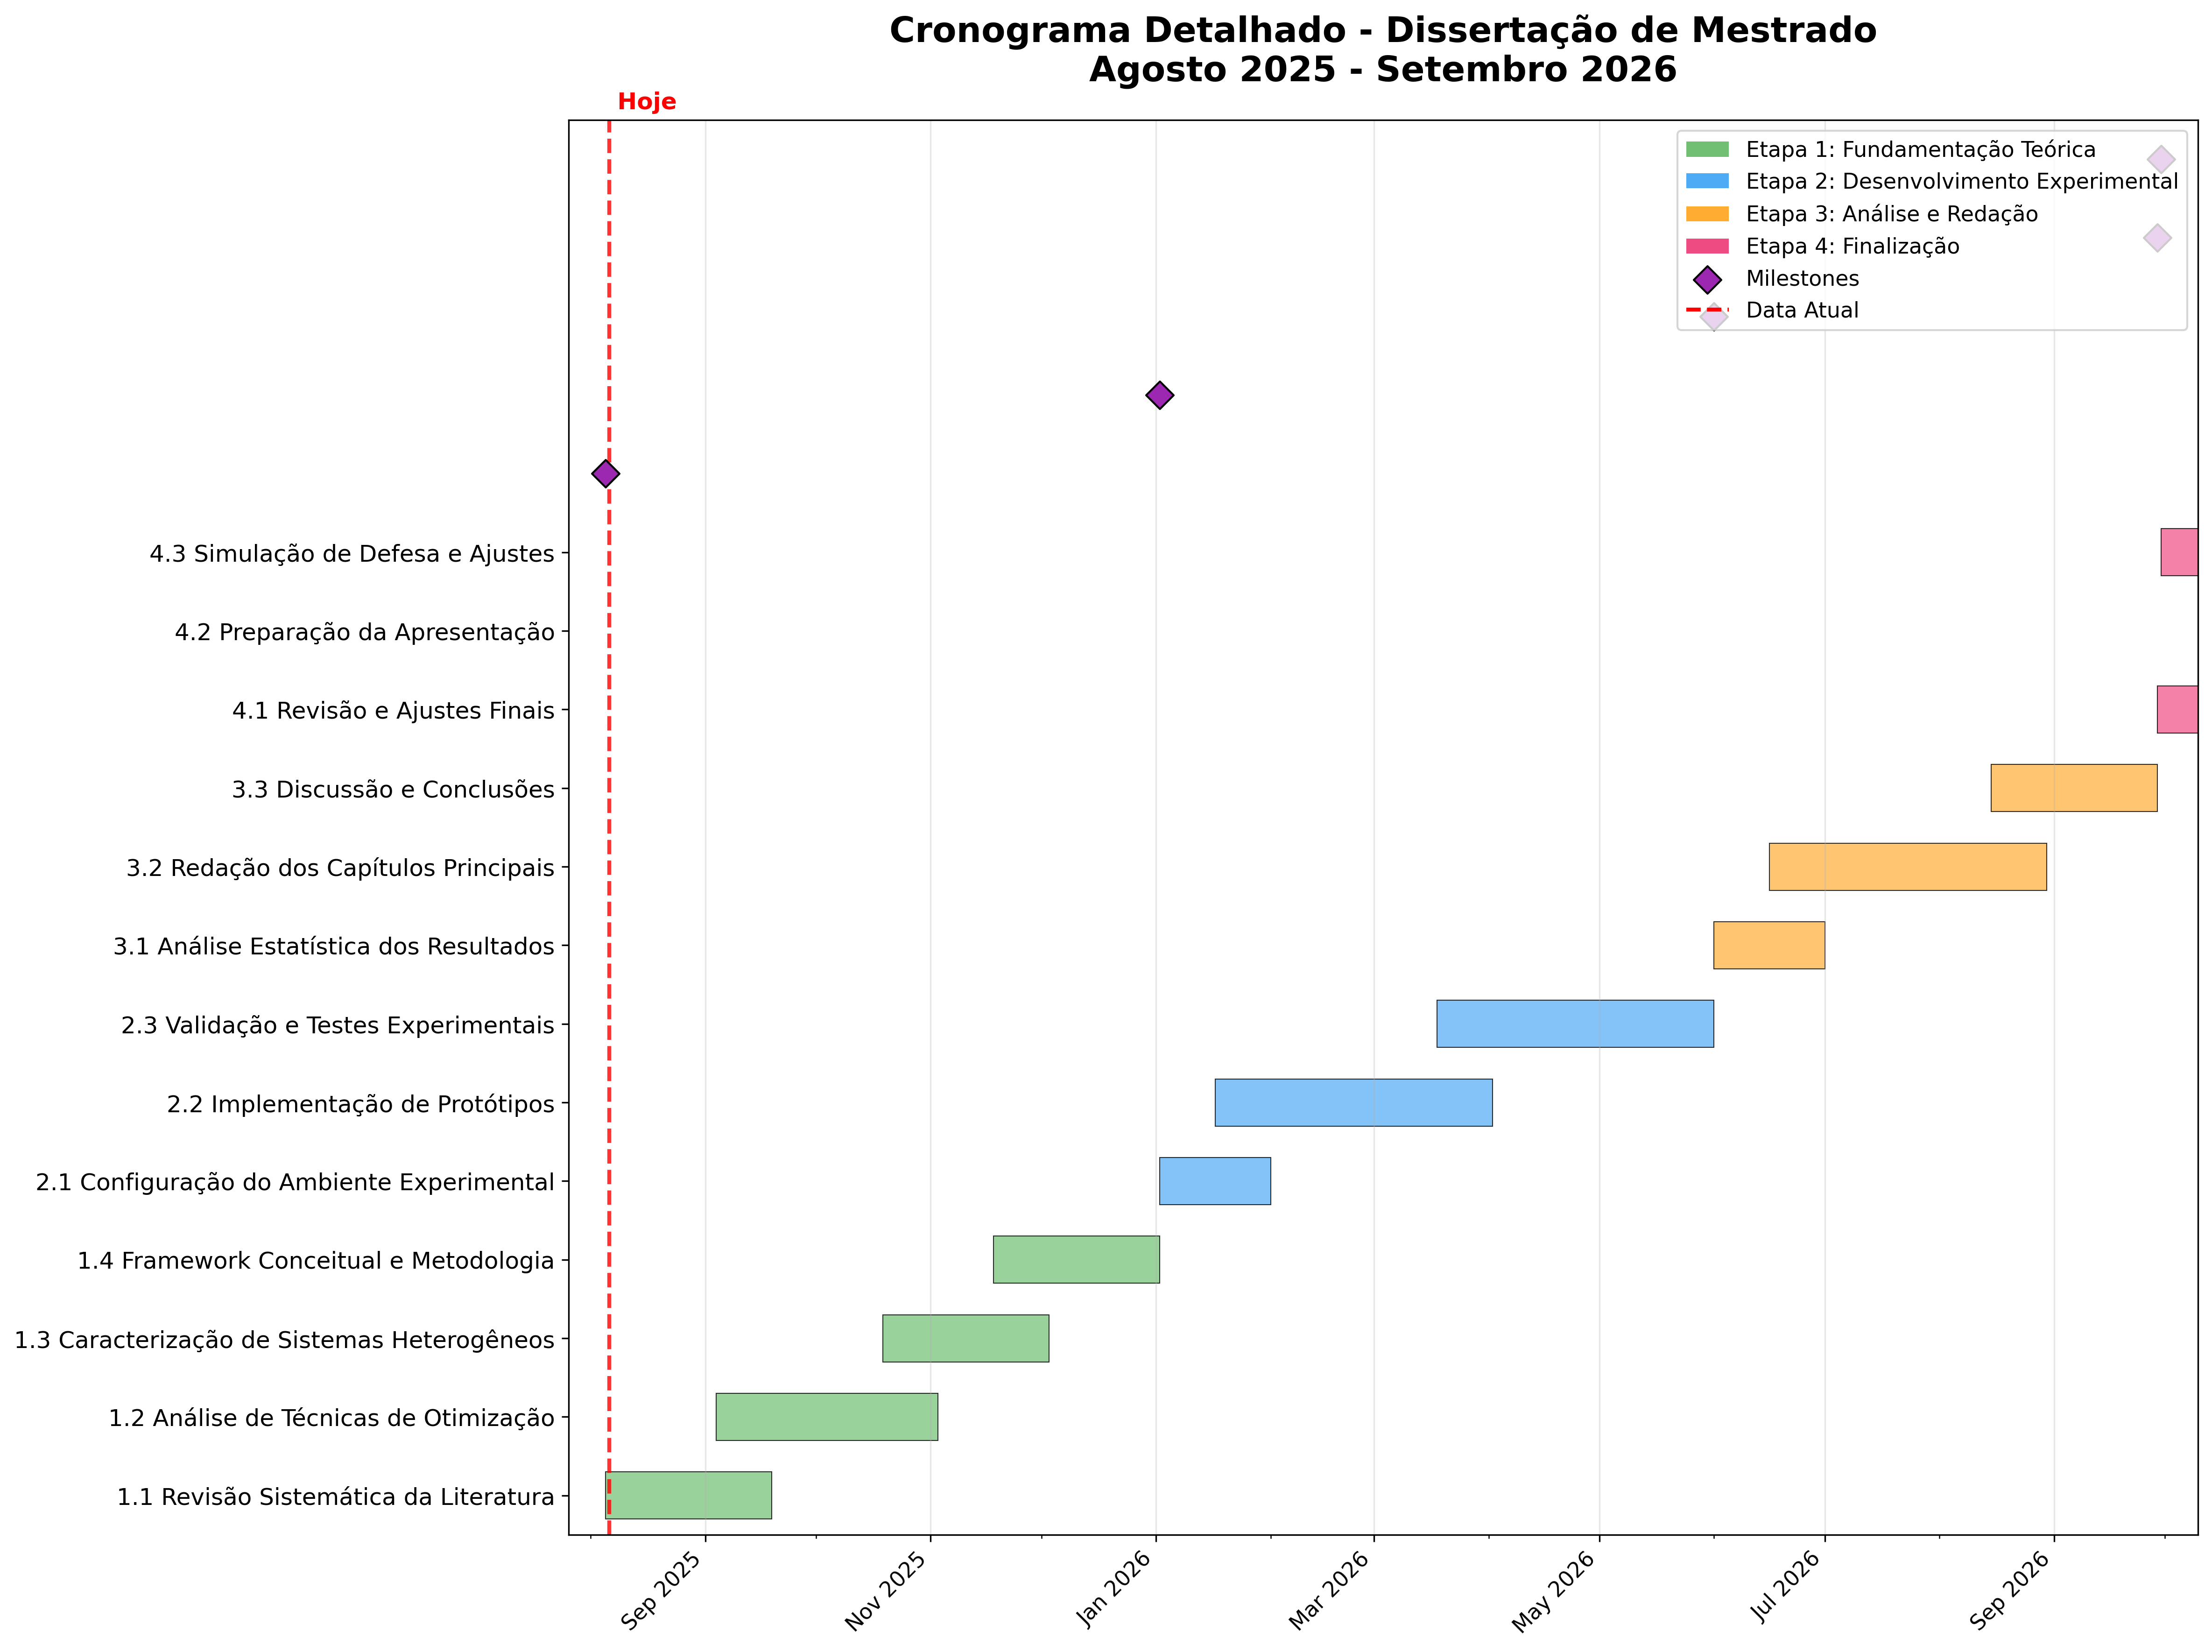
\includegraphics[width=0.95\textwidth]{figuras/cronograma_mestrado_gantt.png}
\caption{Cronograma detalhado do projeto de mestrado (Agosto 2025 - Setembro 2026). O gráfico mostra as quatro etapas principais, 12 tarefas detalhadas e 4 milestones críticos. A linha vermelha pontilhada indica a data atual, permitindo acompanhar o progresso do projeto. As cores representam as diferentes etapas: verde (Fundamentação Teórica), azul (Desenvolvimento Experimental), laranja (Análise e Redação) e rosa (Finalização).}
\label{fig:cronograma}
\end{figure}

\subsection{Etapa 1: Fundamentação Teórica e Estado da Arte (Agosto 2025 - Janeiro 2026)}

\textbf{Duração}: 5 meses (Agosto 2025 - Janeiro 2026)

\textbf{Objetivos Principais}:
\begin{itemize}
\item Revisão sistemática da literatura sobre técnicas de otimização para processamento hiperespectral
\item Análise detalhada de técnicas comprovadas de redução de dados e otimização energética
\item Caracterização de sistemas heterogêneos e suas aplicações em processamento embarcado
\item Desenvolvimento do framework conceitual e metodologia de validação
\end{itemize}

\textbf{Tarefas Detalhadas}:
\begin{enumerate}
\item \textbf{Revisão Sistemática da Literatura} (1.5 meses): Análise de 20+ artigos científicos com catalogação sistemática de técnicas
\item \textbf{Análise de Técnicas de Otimização} (2 meses): Caracterização quantitativa de compressive sensing, seleção EMCR e codesign HW/SW
\item \textbf{Caracterização de Sistemas Heterogêneos} (1.5 meses): Análise de arquiteturas CPU+GPU+FPGA e seus trade-offs
\item \textbf{Framework Conceitual e Metodologia} (1.5 meses): Desenvolvimento da metodologia de validação e especificações técnicas
\end{enumerate}

\textbf{Entregáveis}:
\begin{itemize}
\item Relatório de revisão sistemática com matriz de técnicas catalogadas
\item Framework conceitual para sistemas heterogêneos
\item Metodologia detalhada de validação experimental
\item Baseline teórico para comparação de resultados
\end{itemize}

\subsection{Etapa 2: Desenvolvimento Experimental e Validação (Janeiro - Maio 2026)}

\textbf{Duração}: 5 meses (Janeiro - Maio 2026)

\textbf{Objetivos Principais}:
\begin{itemize}
\item Configuração do ambiente experimental heterogêneo
\item Implementação de protótipos de prova de conceito
\item Validação experimental das técnicas identificadas
\item Quantificação dos trade-offs entre performance, consumo e precisão
\end{itemize}

\textbf{Tarefas Detalhadas}:
\begin{enumerate}
\item \textbf{Configuração do Ambiente Experimental} (1 mês): Setup da plataforma heterogênea e ferramentas de desenvolvimento
\item \textbf{Implementação de Protótipos} (2.5 meses): Desenvolvimento de módulos FPGA, GPU e CPU com integração
\item \textbf{Validação e Testes Experimentais} (2.5 meses): Execução de experimentos e coleta de dados de performance
\end{enumerate}

\textbf{Entregáveis}:
\begin{itemize}
\item Plataforma experimental funcional
\item Protótipos implementados e validados
\item Dados experimentais de performance e consumo
\item Análise preliminar dos resultados
\end{itemize}

\subsection{Etapa 3: Análise de Resultados e Redação (Maio - Agosto 2026)}

\textbf{Duração}: 4 meses (Maio - Agosto 2026)

\textbf{Objetivos Principais}:
\begin{itemize}
\item Análise estatística detalhada dos resultados experimentais
\item Redação dos capítulos principais da dissertação
\item Discussão dos resultados e suas implicações
\item Formulação de conclusões e trabalhos futuros
\end{itemize}

\textbf{Tarefas Detalhadas}:
\begin{enumerate}
\item \textbf{Análise Estatística dos Resultados} (1 mês): Processamento estatístico e validação de significância
\item \textbf{Redação dos Capítulos Principais} (2.5 meses): Escrita dos capítulos de introdução, metodologia e resultados
\item \textbf{Discussão e Conclusões} (1.5 meses): Análise crítica dos resultados e formulação de conclusões
\end{enumerate}

\textbf{Entregáveis}:
\begin{itemize}
\item Análise estatística completa dos resultados
\item Capítulos da dissertação redigidos
\item Discussão crítica dos achados
\item Conclusões e diretrizes para trabalhos futuros
\end{itemize}

\subsection{Etapa 4: Finalização e Preparação para Defesa (Agosto - Setembro 2026)}

\textbf{Duração}: 1.5 meses (Agosto - Setembro 2026)

\textbf{Objetivos Principais}:
\begin{itemize}
\item Revisão e ajustes finais da dissertação
\item Preparação da apresentação de defesa
\item Simulação de defesa e ajustes finais
\item Submissão final e preparação para defesa
\end{itemize}

\textbf{Tarefas Detalhadas}:
\begin{enumerate}
\item \textbf{Revisão e Ajustes Finais} (1 mês): Correção de erros e melhorias na dissertação
\item \textbf{Preparação da Apresentação} (1 mês): Desenvolvimento dos slides e ensaios
\item \textbf{Simulação de Defesa e Ajustes} (1 mês): Prática da apresentação e refinamentos
\end{enumerate}

\textbf{Entregáveis}:
\begin{itemize}
\item Dissertação final revisada e formatada
\item Apresentação de defesa preparada
\item Material de apoio para a banca
\item Documentação completa do projeto
\end{itemize}

\subsection{Milestones Principais}

O cronograma inclui quatro milestones críticos que marcam pontos de verificação importantes:

\begin{enumerate}
\item \textbf{M1: Framework Conceitual Completo} (Janeiro 2026): Conclusão da fundamentação teórica e metodologia
\item \textbf{M2: Protótipos Validados} (Maio 2026): Validação experimental das técnicas propostas
\item \textbf{M3: Dissertação Completa} (Agosto 2026): Documento final redigido e revisado
\item \textbf{M4: Defesa} (Setembro 2026): Apresentação e defesa da dissertação
\end{enumerate}

\subsection{Controle e Acompanhamento}

\textbf{Monitoramento Semanal}:
\begin{itemize}
\item Reuniões de acompanhamento com orientador
\item Atualização do progresso das tarefas
\item Identificação de riscos e ajustes no cronograma
\end{itemize}

\textbf{Revisões Mensais}:
\begin{itemize}
\item Avaliação do progresso geral do projeto
\item Ajustes no cronograma conforme necessário
\item Validação da qualidade dos entregáveis
\end{itemize}

\textbf{Contingências}:
\begin{itemize}
\item Buffer de tempo de 2 semanas em cada etapa para imprevistos
\item Plano alternativo para atrasos em tarefas críticas
\item Flexibilidade na sequência de algumas tarefas paralelas
\end{itemize}

\section{Metodologia de Análise dos Resultados}

\subsection{Análise Estatística}

\textbf{Testes Estatísticos}:
\begin{itemize}
\item ANOVA para comparação entre diferentes configurações
\item Teste t-student para validação de significância das melhorias
\item Análise de correlação entre métricas de trade-off
\end{itemize}

\textbf{Validação de Robustez}:
\begin{itemize}
\item Análise de sensibilidade a variações de parâmetros
\item Teste com diferentes datasets para generalização
\item Avaliação de estabilidade temporal dos resultados
\end{itemize}

\subsection{Comparação com Estado da Arte}

\textbf{Benchmarks de Referência}:
\begin{itemize}
\item Comparação com implementações CPU convencionais
\item Análise relativa às melhores soluções GPU/FPGA da literatura
\item Avaliação do potencial de melhoria teórico vs prático
\end{itemize}

\textbf{Métricas de Comparação}:
\begin{itemize}
\item Fator de melhoria energética (speedup energético)
\item Redução percentual de latência
\item Manutenção/melhoria da precisão
\item Viabilidade de implementação prática
\end{itemize}

% O comando a seguir inclui o arquivo conclusoes.tex
% que contém o capítulo de conclusoes. 
% Detalhe: não precisa incluir a extensão .tex
% Capítulo de Conclusões
\chapter{Conclusões}\label{chp:conclusoes}

Este capítulo apresentará as conclusões finais do trabalho, sintetizando os resultados obtidos na análise comparativa das diferentes arquiteturas computacionais para processamento hiperespectral em tempo real. O conteúdo detalhado será desenvolvido após a conclusão das implementações e análises.

\section{Síntese dos Resultados}\label{sec:sintese}

[Conteúdo a ser desenvolvido]

\section{Contribuições}\label{sec:contribuicoes}

[Conteúdo a ser desenvolvido]

\section{Limitações}\label{sec:limitacoes}

[Conteúdo a ser desenvolvido]

\section{Trabalhos Futuros}\label{sec:trabalhos_futuros}

[Conteúdo a ser desenvolvido]

% O comando condicional \ifturnitin a seguir é importante para 
% preparar o texto para encaminhamento ao Turnitin. 
% NÃO REMOVA!!
% O \fi correspondente está antes do \end{document}
\ifturnitin
    \relax
\else 
% Comandos para incluir as referências bibliográficas
% Define espaçamento simples em cada referência
\begin{singlespacing}

% Adiciona uma linha em branco entre duas referências
\setlength\bibitemsep{10pt}   
%
% Adiciona as referências bibliográficas.
% Mude o título (title), caso o texto seja em inglês 
% ou espanhol.
\printbibliography[heading=bibintoc, % Adiciona no sumário
                   title={Referências bibliográficas} % Nome do Capítulo
                  ]
\end{singlespacing}

% Os anexos, se houver, vêm depois das referências:
\appendix

% O comando a seguir inclui o arquivo apendices.tex
% que contém os apêndices. Observe o comando \appendix
% na linha anterior
% Detalhe: não precisa incluir a extensão .tex
\chapter{Primeiro Apêndice}
% O comando a seguir gera um "dummy text". 
% Elimine-o quando escrever sua dissertação.
\lipsum[9]

\chapter{Segundo  Apêndice}
% O comando a seguir gera um "dummy text". 
% Elimine-o quando escrever sua dissertação.
\lipsum[10]

%
%% O comando \fi a seguir é obrigatório para o controle 
%% da opção "turnitin". Não o remova!!
\fi
\end{document}